\section{Introdução}

\subsection{Contextualização}
% Apresente o USV-Lab como uma plataforma da Marinha do Brasil para pesquisa e desenvolvimento em veículos autônomos marítimos.

A navegação marítima autônoma representa avanços significativos na segurança e eficiência das atividades marítimas. Embora o conceito de navios autônomos não seja recente sua aplicação atual é ampla, com benefícios como a redução de erros humanos e a otimização de recursos. No campo militar, a navegação não tripulada tem ganhado destaque, ampliando capacidades operacionais e mitigando riscos humanos. Nesse contexto, a Marinha do Brasil, com um papel estratégico na defesa da Amazônia Azul, busca desenvolver capacidades de navegação autônoma, especialmente para missões de reconhecimento, por meio do Veículo de Superfície Não Tripulado Laboratorial (VSNT-Lab), exibido na figura~\ref{fig:intro_vsnt}. Essa iniciativa reflete a estratégia da Marinha em explorar o potencial da navegação autônoma para operações táticas avançadas\cite{douglas2024_VSNT}.

\begin{figure}[H]
    \caption{Veículo de Superfície Não Tripulado Laboratorial (VSNT-Lab)}
       \centering
       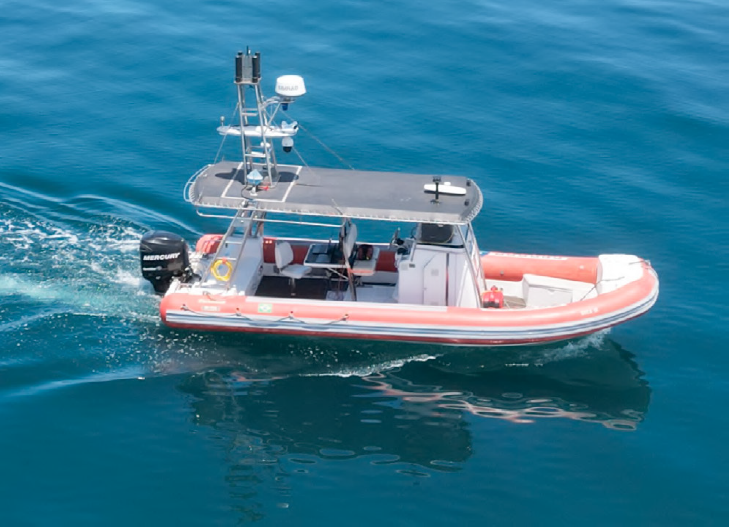
\includegraphics[height=6cm]{figuras/intro_vsnt.png}
       \label{fig:intro_vsnt}
   \small
   
   Fonte: Lima et al. \cite{douglas2024_VSNT}.
   \end{figure}


% Destaque a importância da comunicação eficiente e resiliente em missões autônomas, como as realizadas durante o exercício MINEX-23.
% Explique os desafios de manter comunicações peer-to-peer confiáveis entre o navio-mãe e o USV-Lab em cenários de operações críticas.

\subsection{Problema}
% Identifique problemas como latência, perda de pacotes e falhas de comunicação em canais mesh e VPN, que comprometem a autonomia e a eficiência das missões.

\subsection{Justificativa}
% Ressalte como a pesquisa contribui para a robustez das operações autônomas e para a segurança em missões militares e civis, alinhada aos interesses estratégicos da Marinha no "Amazônia Azul".